\documentclass[fontsize=10pt]{scrartcl}

\usepackage{enumitem}
	\setenumerate{listparindent=\parindent}
\usepackage{amsmath}
\usepackage{amssymb}
\usepackage{graphicx}
\usepackage{placeins}
\usepackage{hyperref}
\usepackage{float}
\usepackage[hyphenbreaks]{breakurl}
\usepackage[margin=1.0in]{geometry}

\newcommand{\code}{\texttt}

\begin{document}

	\title{CSC 522 : Automated Learning and Data Analysis}
	\subtitle{Homework 3}
	\author{Roopak Venkatakrishnan - rvenkat7@ncsu.edu}
	\maketitle

	\section{Question 1}
	Devise a training set for use as input to the ID3 algorithm in order to produce a decision tree with a particular structure. We’re providing the required target decision tree that should be induced using your training set. In other words, instead of the usual tree induction learning problem where we’re given training data and a tree learner and we see what the program outputs, for this assignment you are given the desired output, and must design the input to produce it. To test your candidate training sets, you may use either Weka, Matlab or R.

	Construct a training set having the appropriate format for the classifier you are using, which, when used with the classifier, comes as close as you can to outputting the given decision tree. The decision tree:
\begin{verbatim}
tear-prod-rate=(normal)
| astigmatism=(yes)
| | spectacle-prescrip=(hypermetrope): none
| | spectacle-prescrip!=(hypermetrope): hard
| astigmatism!=(yes)
| | age=(presbyopic): soft
| | age!=(presbyopic): soft
tear-prod-rate!=(normal): none

\end{verbatim}

	``Outputting the tree'' means the tree structure is the same as above, with the same decision nodes in the same places, etc. Generating just any tree, no matter how accurate, is not sufficient. There must be no missing data in your training set. In other words, each example must have values for all attributes. For each example, the training set should provide values for all the following attributes, including the attributes that do not appear in the target tree. The list of attributes is given in Table 1.

	\textbf{Deliverables:} Turn in the following:
	\begin{enumerate}
	\item
	A description of how you arrived at the dataset. An answer along the lines of “I got lucky” or “this was simple trial and error” are not acceptable.

	\item
	A description of how to load the dataset in either Matlab, Weka or R, and the toolbox or package used.

	\item
	A text file with the dataset you generated.
	\end{enumerate}

	\begin{table}[H]
		\centering
	    \begin{tabular}{|c|c|}
                          \hline
	        Attributes                    & Values                            	\\ \hline \hline
	        age                           & \{young,pre-presbyopic,presbyopic\} \\ 
	        spectacle-prescrip            & \{hypermetrope,myope\}              \\ 
	        astigmatism                   & \{yes,no\}                          \\ 
	        tear-prod-rate                & \{reduced,normal\}                  \\ 
	        contact-lenses (Target Class) & \{none,soft,hard\}                  \\ 
                          \hline
                      \end{tabular}
        \caption{Table with attributes and values}
	\end{table}

	\textbf{Arriving At the dataset}

	We notice that tear-prod-rate is the root of the tree. So we try to center our values in such a way that they revolve around tear-prod-rate. The first branch says that if tear-prod-rate is reduced then the lenses required are none. We try and depict this in such a way that contact-lenses depends on nothing else but the tear-prod-rate. To achieve this we add all possible combinations of astigmatism,spectacle-prescrip and age. This way no pattern is formed here and looking at the data the ID3 algorithm is forced to say when tear-prod-rate is reduced then contact lenses is none. If we do not account for all combinations some other pattern may for unbeknown to us.

	Next we work on the other branch of the tree, where tear-prod-rate is normal. Now we see that astigmatism is the next branch. Let us consider the case where astigmatism is yes. We notice that if spectacle-prescrip=hypermetrope the contact-lense is none otherwise it is hard. So we work combinations in such way that we keep tear-prod-rate=normal, astigmatism=yes and spectacle-prescrip=hypermetrope we set cpntact-lense to none for all possible values of age. This ensures that age doesnt contribute to a pattern at this point. Next we consider tear-prod-rate=normal, astigmatism=yes and spectacle-prescrip=myope and set contact-lense=hard for all possible values of age. This makes sue that at this point the tree is split only the way we want it to be split and random patterns dont develop without our notice.

	Next we work on the branch where astigmatism is no. we consider tear-prod-rate=normal, astigmatism=no and age=presbyopic. For this we set spectacle-prescrip to all possible values and set the contact-lense=soft. This way the only pattern is that of tear-prod-rate->astigmatism->age(presbyopic). For the other two values of age (young and pre-presbyopic) we set all possible values of spectacle-prescrip for each of them. 

	We have thus constructed an ID3 algorithm in such a way that it is forced to go the way we want it to go. Because all other cases would end up with a tree of much higher length.

	The exact tree generated by my algorithm is as shown below.

\begin{verbatim}
tear-prod-rate = normal
|  astigmatism = yes
|  |  spectacle-prescrip = hypermetrope: none
|  |  spectacle-prescrip = myope: hard
|  astigmatism = no
|  |  age = pre-presbyopic: none
|  |  age = presbyopic: soft
|  |  age = young: none
tear-prod-rate = reduced: none
\end{verbatim}


	\textbf{Loading My Dataset}
	This dataset was designed to be used with Weka. The steps are as follows.
	\begin{itemize}
		\item
		Run Weka

		\item
		Click on Explorer

		\item
		Navigate to the ``Preprocess'' tab.

		\item
		Click Open-File and navigate to the file. (file-type csv)

		\item
		Go to the clasify tab, choos filter as Id3

		\item
		Make sure contact-lenses is selected in the drop down (Nom)

		\item
		leave the Test options unchanged. and click start

		\item
		Result is produced on the classifier output box in the same tab.
	\end{itemize}
	\section{Question 2}

		\begin{sloppypar}
		For this exercise, we will use the Balloons dataset (\url{http://archive.ics.uci.edu/ml/datasets/Balloons}). Specifically, we will use the yellow-small+adult-stretch data. (\burl{http://archive.ics.uci.edu/ml/machine-learning-databases/balloons/yellow-small+adult-stretch.data}).
		\end{sloppypar}
		The data has 16 entries each four attributes, all of which are nominal. Each entry belongs to one of the two classes {T, F}. Complete the following tasks.

		\begin{enumerate}
			\item
			Compute the tree using Gini index. Show all necessary calculations.

\begin{verbatim}
> vals<-read.csv(file.choose())
> names(vals)<- c("color","size","act","age","inflated")
> findgini <- function (vals, inflated) {
+   
+   
+     unq <- unique(vals)
+     gini <- c()
+     df <- data.frame(v=vals,inf=inflated)
+     gini_final<-0
+     for(i in 1:length(unq))
+     {
+       no_type_i <- length(vals[which(vals==unq[i])])
+       no_true <- length(which(inflated[which(vals==unq[i])]))
+       no_false <- no_type_i - no_true
+       tmp = 1 -(no_true/no_type_i)^2 -(no_false/no_type_i)^2
+       tlength <-length(vals)
+       gini_final<-gini_final + ((no_type_i/tlength)*tmp)
+     }
+     print(paste("The Gini is ",gini_final))
+   
+ 
+ }
> findgini(vals$color,vals$inflated)
[1] "The Gini is  0.421875"
> findgini(vals$size,vals$inflated)
[1] "The Gini is  0.421875"
> findgini(vals$act,vals$inflated)
[1] "The Gini is  0.421875"
> findgini(vals$age,vals$inflated)
[1] "The Gini is  0.421875"
> findgini(vals$size[which(vals$color=="YELLOW")],
+ vals$inflated[which(vals$color=="YELLOW")])
[1] "The Gini is  0.1875"
> findgini(vals$act[which(vals$color=="YELLOW")],
+ vals$inflated[which(vals$color=="YELLOW")])
[1] "The Gini is  0.4375"
> findgini(vals$age[which(vals$color=="YELLOW")],
+ vals$inflated[which(vals$color=="YELLOW")])
[1] "The Gini is  0.4375"
> findgini(vals$size[which(vals$color=="PURPLE")],
+ vals$inflated[which(vals$color=="PURPLE")])
[1] "The Gini is  0.375"
> findgini(vals$act[which(vals$color=="PURPLE")],
+ vals$inflated[which(vals$color=="PURPLE")])
[1] "The Gini is  0.25"
> findgini(vals$age[which(vals$color=="PURPLE")],
+ vals$inflated[which(vals$color=="PURPLE")])
[1] "The Gini is  0.25"
> findgini(vals$act[intersect(which(vals$color=="YELLOW"),
+ which(vals$size=="SMALL"))],
+ vals$inflated[intersect(which(vals$color=="YELLOW"),
+ which(vals$size=="SMALL"))])
[1] "The Gini is  0"
> findgini(vals$act[intersect(which(vals$color=="YELLOW"),
+ which(vals$size=="LARGE"))],
+ vals$inflated[intersect(which(vals$color=="YELLOW"),
+ which(vals$size=="LARGE"))])
[1] "The Gini is  0.25"
> findgini(vals$age[intersect(which(vals$color=="YELLOW"),
+ which(vals$size=="LARGE"))],
+ vals$inflated[intersect(which(vals$color=="YELLOW"),
+ which(vals$size=="LARGE"))])
[1] "The Gini is  0.25"
> findgini(vals$age[intersect(which(vals$color=="YELLOW"),
+ which(vals$size=="SMALL"))],
+ vals$inflated[intersect(which(vals$color=="YELLOW"),
+ which(vals$size=="SMALL"))])
[1] "The Gini is  0"
> findgini(vals$age[intersect(which(vals$color=="YELLOW"),
+ which(vals$size=="LARGE"))],
+ vals$inflated[intersect(which(vals$color=="YELLOW"),
+ which(vals$size=="LARGE"))])
[1] "The Gini is  0.25"
> findgini(vals$size[intersect(which(vals$color=="PURPLE"),
+ which(vals$act=="STRETCH"))],
+ vals$inflated[intersect(which(vals$color=="PURPLE"),
+ which(vals$act=="STRETCH"))])
[1] "The Gini is  0.5"
> findgini(vals$age[intersect(which(vals$color=="PURPLE"),
+ which(vals$act=="STRETCH"))],
+ vals$inflated[intersect(which(vals$color=="PURPLE"),
+ which(vals$act=="STRETCH"))])
[1] "The Gini is  0"
> findgini(vals$age[intersect(which(vals$color=="PURPLE"),
+ which(vals$act=="DIP"))],
+ vals$inflated[intersect(which(vals$color=="PURPLE"),
+ which(vals$act=="DIP"))])
[1] "The Gini is  0"
> findgini(vals$act[intersect(which(vals$color=="PURPLE"),
+ which(vals$act=="DIP"))],
+ vals$inflated[intersect(which(vals$color=="PURPLE"),
+ which(vals$act=="DIP"))])
[1] "The Gini is  0"
\end{verbatim}
			Let us use the above function and the data to construct a decision tree. This function computes the Gini value given the corresponding values and the respective output expected.

			First we see wehere we get the lowest $GINI_{split}$ trying all columns. In this case we notice that all the columns give us a value of $GINI_{split} = 0.421875$. This value is calculated by the above written fucntion.\\
			Let us run through how the function calculates the $GINI_{split}$. First it finds GINI for each of the different values of the column passed. Let us consider as an exmaple. It has two different values, YELLOW and PURPLE. Let us now calulate GINI(color=YELLOW).

			This can be found as 
			\begin{equation*}
				1 - (\frac{5}{8})^{2} - (\frac{3}{8})^{2}
			\end{equation*}

			Similarly  we find the GINI value for PURPLE

			Combining both the values given we find the value for $GINI_{split} (Color)$

			Since our function does the abve steps we can use the value it gives us and move forward quicker.

			Since all seem to have the same level of impurity in the firts level, let us just pick color move on.\\
			Now we try and see what happens for color = YELLOW and size,act,age. We see the following.\\


			Given COLOR=YELLOW, $GINI_{split}$ is given to be
			\[   \left\{
                  \begin{array}{ll}
                        0.1875 & size \\
                        0.4375 & act \\
                        0.4375 & age \\
                  \end{array} 
                  \right. \]
			
			Given COLOR =PURPLE, $GINI_{split}$ is given to be
			\[   \left\{
                  \begin{array}{ll}
                        0.375 & size \\
                        0.25 & act \\
                        0.25 & age \\
                  \end{array} 
                  \right. \]
            Given the above we can see the best partition would be along size for COLOR=YELLOW and either of act/age for COLOR=PURPLE. Let us choose to proceed with act for PURPLE

            Given COLOR=YELLOW, SIZE=LARGE, $GINI_{split}$ is found to be
            \[   \left\{
                  \begin{array}{ll}
                        0.25 & act \\
                        0.25 & age \\
                  \end{array} 
                  \right. \]
            Thus since both are identical we can choose either and proceed. From this point onward we find the GINI values to be 0. So we proceed to draw the tree.

            Given COLOR=PURPLE,act=STRETCH, $GINI_{split}$ is found to be
             \[   \left\{
                  \begin{array}{ll}
                        0.5 & size \\
                        0.0 & age \\
                  \end{array} 
                  \right. \]
            Here we choose age and finalize the tree. 

            The final tree we construct looks as follows. \\
            \begin{figure}[H]
				\begin{center}
					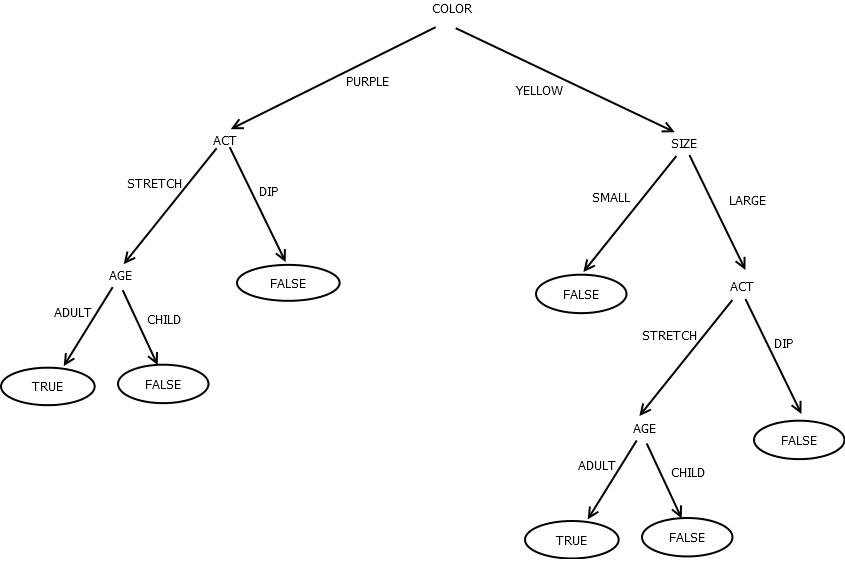
\includegraphics[width=\textwidth]{resources/q2_img1.png}
					\caption{Decision Tree - GINI index}
				\end{center}
			\end{figure}

			\item
			Compute the tree using ID3 entropy computations. Show all necessary calculations.

			The entropy of the entire system is calculated as $-\frac{9}{16}log_{2}(\frac{9}{16}) - \frac{9}{16}log_{2}(\frac{9}{16})$ which comes out to be 0.988. Note however since we are lookig for relative entropy to choose attributes we could assume system=1 and still pick the correct atrribute.

			The following Code finds the entropy of the input.
\begin{verbatim}
> findentropy <- function (vals, inflated,ent_parent) {
+   
+   
+   unq <- unique(vals)
+   gini <- c()
+   df <- data.frame(v=vals,inf=inflated)
+   entropy_final<-0
+   for(i in 1:length(unq))
+   {
+     no_type_i <- length(vals[which(vals==unq[i])])
+     no_true <- length(which(inflated[which(vals==unq[i])]))
+     no_false <- no_type_i - no_true
+     if(no_true!=0 && no_false!=0)
+     {
+       tmp =  -(no_true/no_type_i)*log2(no_true/no_type_i) -
+ (no_false/no_type_i)*log2(no_false/no_type_i)
+     }
+     else if(no_true==0)
+     {
+       tmp = -(no_false/no_type_i)*log2(no_false/no_type_i)
+     }
+     else
+     {
+       tmp = -(no_true/no_type_i)*log2(no_true/no_type_i)
+     }
+     tlength <-length(vals)
+     entropy_final<-entropy_final + ((no_type_i/tlength)*tmp)
+   }
+   entf<- ent_parent-entropy_final
+   print(paste("The Entropy is ",entf))
+   
+   
+ }
> findentropy(vals$color,vals$inflated,.988)
[1] "The Entropy is  0.105143936307951"
> findentropy(vals$siz,vals$inflated,.988)
[1] "The Entropy is  0.105143936307951"
> findentropy(vals$size,vals$inflated,.988)
[1] "The Entropy is  0.105143936307951"
> findentropy(vals$act,vals$inflated,.988)
[1] "The Entropy is  0.105143936307951"
> findentropy(vals$age,vals$inflated,.988)
[1] "The Entropy is  0.105143936307951"
\end{verbatim}

		Since they are all similar We choose, color and proceed. \\
		The entropy of the system on the yellow side is 0.95 \\
\begin{verbatim}
> findentropy(vals$size[which(vals$color=="YELLOW")],
+ vals$inflated[which(vals$color=="YELLOW")],.95)
[1] "The Entropy is  0.544360937770433"
> findentropy(vals$act[which(vals$color=="YELLOW")],
+ vals$inflated[which(vals$color=="YELLOW")],.95)
[1] "The Entropy is  0.0443609377704335"
> findentropy(vals$age[which(vals$color=="YELLOW")],
+ vals$inflated[which(vals$color=="YELLOW")],.95)
[1] "The Entropy is  0.0443609377704335"
\end{verbatim}
		
		Given the entropy values we pick size and go on.
		We may also note that we can consider the entropy of the system to be 1 for all nodes while splitting as we only try and find the relative value.
\begin{verbatim}
> findentropy(vals$act[intersect(which(vals$color=="YELLOW"),
+ which(vals$size=="SMALL"))],
+ vals$inflated[intersect(which(vals$color=="YELLOW"),
+ which(vals$size=="SMALL"))],1)
[1] "The Entropy is  1"
> findentropy(vals$act[intersect(which(vals$color=="YELLOW"),
+ which(vals$size=="LARGE"))],
+ vals$inflated[intersect(which(vals$color=="YELLOW"),
+ which(vals$size=="LARGE"))],1)
[1] "The Entropy is  0.5"
> findentropy(vals$age[intersect(which(vals$color=="YELLOW"),
+ which(vals$size=="LARGE"))],
+ vals$inflated[intersect(which(vals$color=="YELLOW"),
+ which(vals$size=="LARGE"))],1)
[1] "The Entropy is  0.5"
\end{verbatim}
		Now we see that the data for Yellow and small is classified, however we know have to pick etween act and age both which have the same entropy. Let us pick act and move on.

\begin{verbatim}
> findentropy(vals$age[intersect(intersect(which(vals$color=="YELLOW"),
+ which(vals$size=="LARGE")),which(vals$act=="DIP"))],
+ vals$inflated[intersect(intersect(which(vals$color=="YELLOW"),
+ which(vals$size=="LARGE")),which(vals$act=="DIP"))],1)
[1] "The Entropy is  1"
> findentropy(vals$age[intersect(intersect(which(vals$color=="YELLOW"),
+ which(vals$size=="LARGE")),which(vals$act=="STRETCH"))],
+ vals$inflated[intersect(intersect(which(vals$color=="YELLOW"),
+ which(vals$size=="LARGE")),which(vals$act=="STRETCH"))],1)
[1] "The Entropy is  1"
> findentropy(vals$act[intersect(intersect(which(vals$color=="YELLOW"),
+ which(vals$size=="LARGE")),which(vals$act=="DIP"))],
+ vals$inflated[intersect(intersect(which(vals$color=="YELLOW"),
+ which(vals$size=="LARGE")),which(vals$act=="DIP"))],1)
[1] "The Entropy is  1"
\end{verbatim}
		From the values we can see that considering  yellow large an stretch the data can be classified further. But since we have only one remaining attribute  we have constructed this part of the tree.

Now moving to the other part of the tree.

\begin{verbatim}
> findentropy(vals$size[which(vals$color=="PURPLE")],
+ vals$inflated[which(vals$color=="PURPLE")],1)
[1] "The Entropy is  0.188721875540867"
> findentropy(vals$act[which(vals$color=="PURPLE")],
+ vals$inflated[which(vals$color=="PURPLE")],1)
[1] "The Entropy is  0.5"
> findentropy(vals$age[which(vals$color=="PURPLE")],
+ vals$inflated[which(vals$color=="PURPLE")],1)
[1] "The Entropy is  0.5"
\end{verbatim}
		We pick act and now try and move on.

\begin{verbatim}	
> findentropy(vals$size[intersect(which(vals$color=="PURPLE"),
+ which(vals$act=="DIP"))],
+ vals$inflated[intersect(which(vals$color=="PURPLE"),
+ which(vals$act=="DIP"))],1)
[1] "The Entropy is  1"
> findentropy(vals$age[intersect(which(vals$color=="PURPLE"),
+ which(vals$act=="DIP"))],
+ vals$inflated[intersect(which(vals$color=="PURPLE"),
+ which(vals$act=="DIP"))],1)
[1] "The Entropy is  1"
\end{verbatim}
		This means that we have to work with stretch as dip is classifed

		Using the data we can see that choosing age with stretch we can classify the remaingin data.
\begin{verbatim}
> findentropy(vals$size[intersect(which(vals$color=="PURPLE"),
+ which(vals$act=="STRETCH"))],
+ vals$inflated[intersect(which(vals$color=="PURPLE"),
+ which(vals$act=="STRETCH"))],1)
[1] "The Entropy is  0"
> findentropy(vals$age[intersect(which(vals$color=="PURPLE"),
+ which(vals$act=="STRETCH"))],
+ vals$inflated[intersect(which(vals$color=="PURPLE"),
+ which(vals$act=="STRETCH"))],1)
[1] "The Entropy is  1"
\end{verbatim}
		
		The tree we have obtained is depicted as follows.
		\begin{figure}[H]
			\begin{center}
				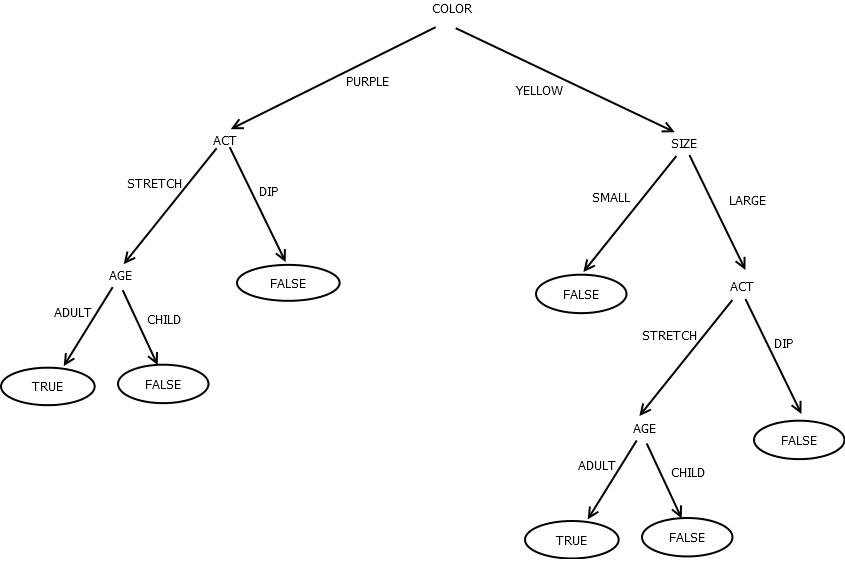
\includegraphics[width=\textwidth]{resources/q2_img1.png}
				\caption{Decision Tree - ID3 Algorithm}
			\end{center}
		\end{figure}

		\item
		Are the trees different? Why? If the trees are different, state which tree is better, and why. Your reasoning must be independent of the test set provided. That is, it must not be along the lines of ``Tree A gives better accuracy on the test set than Tree B''.

		The trees we get from both the algorithms seem to be the same. Since they are the same we cannot say any one of the algorithms is better. However if we have different data sets which give us differnt trees on these algorithms we may be able to compare the trees.

		\item
		Use yellow-small data set as the test set and compute the confusion matrix in each case. If the trees are the same, one confusion matrix is enough, of course.

		The confusion Matrix we get is below.
		\begin{figure}[H]
			\begin{center}
				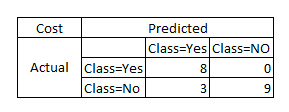
\includegraphics[scale=1]{resources/q2_conf.png}
				\caption{Confusion Matrix}
			\end{center}
		\end{figure}

		\begin{itemize}
			\item
			True Positive -8

			\item
			False Positive - 3

			\item
			True Negative - 9

			\item
			False Negative - 0
		\end{itemize}

		\end{enumerate}

	\section{Question 3}
		Classifiers such as decision trees, neural networks, naive bayes, and many others estimate the conditional probability of class membership. For standard two-class classification problems, the goal is to create a decision procedure that minimizes some notion of prediction error. There are many metrics that measure this, but the ‘naive’ optimal decision for all metrics in this case is:\\
		\[ \hat{y} =    \left\{
                  \begin{array}{ll}
                        1 & : P(y=1|X) > 0.5 \\
                        0 & : P(y=1|X) \leq 0.5 \\
                  \end{array} 
                  \right. \]

        where, $\hat{y}$ is the predicted class, `0' or `1', and P(y = 1|X) is the estimated probability of class membership providedby the classifier.

        This is just a technical way of saying that we will predict the most likely class. This is the optimal rule if the cost of making any decision is the same or if the cost function is ``symmetric''. In this problem we will investigate what happens if the cost function is not symmetric. In a non-symmetric cost function, the penalty associated with misclassification can be different for false negative and false positive predictions, depending on the domain. Pretend you have been approached by a large credit card company. They would like for you to help improve their current fraud detection scheme. They have a wealth of data on consumer transactions that they have used to develop a fraud classifier. This classifier takes as input data on the customer requesting the transaction and the specifics of the transaction such as time, location, and many other details. The classifier outputs an estimated probability that the transaction is fraudulent.

        However, for the credit card company the cost of every decision is not the same. These costs are summarized in Table 2 below. If the transaction is fraudulent and is not caught, the credit card company loses the entire transaction amount. Similarly, if the company decides to decline a transaction because they think it is fraudulent but it is not, the customer may be upset and close their account or use it less in the future, costing the credit card company money.

        \begin{table}[H]
			\centering
		    \begin{tabular}{|c|c|c|c|}
	                          \hline
			        ~  & Prediction        & Truth                  & Cost                         \\ \hline
			        1. & Predict No Fraud  & Transaction Fraudulant & Transaction Amount ($T_{i}$) \\ 
			        2. & Predict Fraud     & Transaction Legitimate & $10 + 0.05 * T_{i}$          \\ 
			        3. & Fraud or No Fraud & Correct                & 0                            \\ 
	                          \hline
	                      \end{tabular}
	        \caption{Cost of Classification}
		\end{table}

		Using this setup, you will be asked to derive the optimal decision rule and compare it to the naive rule. Download the file \texttt{fraud\_probs.csv}. This file contains information on 152880 transactions. The 3 columns are the transaction amount, the estimated probability of fraud from the classifier, and whether or not the transaction was later reported to be fraudulent. A `1' in the 3rd columns means there was fraud while a `0' means there was none.

		\begin{enumerate}
			\item
			Compute the cost of `doing nothing', i.e. always predicting `0', or predicting ``No Fraud'' using the cost matrix given above.

			The cost of doing nothing and predicting 0 all the time is the cost for all transactions where we predicted no fraud but there was a fraud. Which from the table given aboe is the cost fo the transaction. Thus if we find the sum of the trasactions where there was a fraud we have found the cost of predicting ``No Fraud'' all the time.

\begin{verbatim}
> fraud <- read.csv(file.choose())
> sum(fraud$Transaction_Amount[which(fraud$Fraud==1)])
[1] 311347.1
\end{verbatim}
			
			\item
			Calculate the cost of using the naive rule, i.e. predicting `1' when the probability of fraud is \texttt{> 0.5}.

\begin{verbatim}
> fraud$pred <- ifelse(fraud$Probability>.5,1,0)
> fraud$sub <-fraud$Fraud - fraud$pred
> fraud$cost <- ifelse(fraud$sub==1,fraud$Transaction_Amount,
+ ifelse(fraud$sub==-1,(10 + (.05*fraud$Transaction_Amount)),0))
> sum(fraud$cost)
[1] 158855.2
\end{verbatim}
			\textbf{Cost of Naive rule : 158855.2}

			\item
			Calculate the average False Positive cost and the average False Negative cost. To compute the average false positive cost, compute what the cost would be if you made a false positive mistake for every transaction in the data set and then take the average. Repeat this procedure to determine the average false negative cost.

			\textbf{Average False Positive}
\begin{verbatim}
> fraud$cost <-10+(.05*fraud$Transaction_Amount)
> mean(fraud$cost)
[1] 14.5531
\end{verbatim}

			\textbf{Avergae False Negative}
\begin{verbatim}
> fraud$cost <-fraud$Transaction_Amount
> mean(fraud$cost)
[1] 91.06195
\end{verbatim}

		\item
		Now let’s see if we can do better than the naive rule. Let us say for a given transaction and an estimate from the classifier that the transaction is fraudulent, pi, we decide to predict fraud and decline the transaction. What is the expected cost of this decision? Expected cost is defined below: 
		\begin{center}
			(probability decision is correct)*(cost if you are correct) +(probability decision is wrong)*(cost if you are wrong)
		\end{center}
		Please use the established notation in answering this. This should be a function of pi and the costs given in Table 2.

		In this case we have to consider every transaction is a fraud and find the cost.  This is calculated as $10 + .05 \times T_{i}$.
		Further the probability of wrong decision is $1-P_{i}$ here because $P_{i}$ represents the probability of fraud.

\begin{verbatim}
> vals <-read.csv(file.choose())
> vals$pr_wrong <-1 - vals$Probability
> vals$cost <-10+(.05*vals$Transaction_Amount)
> vals$expcost <- vals$pr_wrong * vals$cost
\end{verbatim}

		\item
		What if instead we decided to predict that the same transaction was legitimate (i.e. not fraudulent) and accept the transaction. Using the same fraud probability estimate, $P_{i}$, what is the expected cost in this case?

		In this case, we always predict legitimate and the probability of being wrong is $P_{i}$.

\begin{verbatim}
> vals$cost2 <-vals$Transaction_Amount
> vals$expcost2 <- vals$cost2 * vals$Probability
\end{verbatim}

		\item
		For every transaction, compute the cost for predicting fraud (1) or no fraud (0) using the expected costs from (4) and (5). For each transaction, predict the class with the lower expected cost. Compute the total cost using this procedure and compare it to the cost of the naive rule in (2).

		Using the data calculated above. We just choose the minimum from each cost and sum it up.

\begin{verbatim}
> vals$minecost <-mapply(min,vals$expcost,vals$expcost2)
> sum(vals$minecost)
[1] 63913.12
\end{verbatim}

This value seems to be much lower for cost than what we found using the naive rule. This shows that this a better way of prediction. This model is a better model as we try to minize our cost.
		\end{enumerate}
		
\end{document}